% !TEX encoding = UTF-8
% !TEX TS-program = pdflatex
% !TEX root = ../tesi.tex
% !TEX spellcheck = it-IT
%
%**************************************************************
%/chapter{Progettazione e codifica}
%/label{cap:progettazione-codifica}
%**************************************************************
%
%/intro{Breve introduzione al capitolo}/\
%
%**************************************************************
%/section{Tecnologie e strumenti}
%/label{sec:tecnologie-strumenti}
%
%Di seguito viene data una panoramica delle tecnologie e strumenti utilizzati.
%
%/subsection*{Tecnologia 1}
%Descrizione Tecnologia 1.
%
%/subsection*{Tecnologia 2}
%Descrizione Tecnologia 2
%
%**************************************************************
%/section{Ciclo di vita del software}
%/label{sec:ciclo-vita-software}
%
%**************************************************************
%/section{Progettazione}
%/label{sec:progettazione}
%
%/subsubsection{Namespace 1} %**************************
%Descrizione namespace 1.
%
%/begin{namespacedesc}
    %/classdesc{Classe 1}{Descrizione classe 1}
    %/classdesc{Classe 2}{Descrizione classe 2}
%/end{namespacedesc}
%
%
%**************************************************************
%/section{Design Pattern utilizzati}
%
%**************************************************************
%/section{Codifica}
%**************************************************************
\chapter{Il modulo clienti}
\label{cap:modulo-clienti}
%**************************************************************

\intro{In questo capitolo verrà esposta l'implementazione e le fasi che hanno portato la creazione del modulo clienti}\\

\section{Scopo del modulo} il modulo clienti si pone come scopo quello di creare un semplice sistema di CRUD in un database. In questo caso è stato implementato in un database Postgres, che è quello che viene incluso di default con la distribuzione di Alfresco Community, ma è stata esplicita richiesta dell'azienda che fosse possibile una configurazione su ambienti simili ma che non fossero esclusivamente Postgres.
\section{Presentazione generale del modulo}
Nella figura \ref{fig:cartelle-clienti} si illustra in generale quanto è stato prodotto per questo modulo. In seguito, nella descrizione di dettaglio, si indicheranno i nomi specifici di tutti i file creati
\begin{figure}[!ht]
\centering
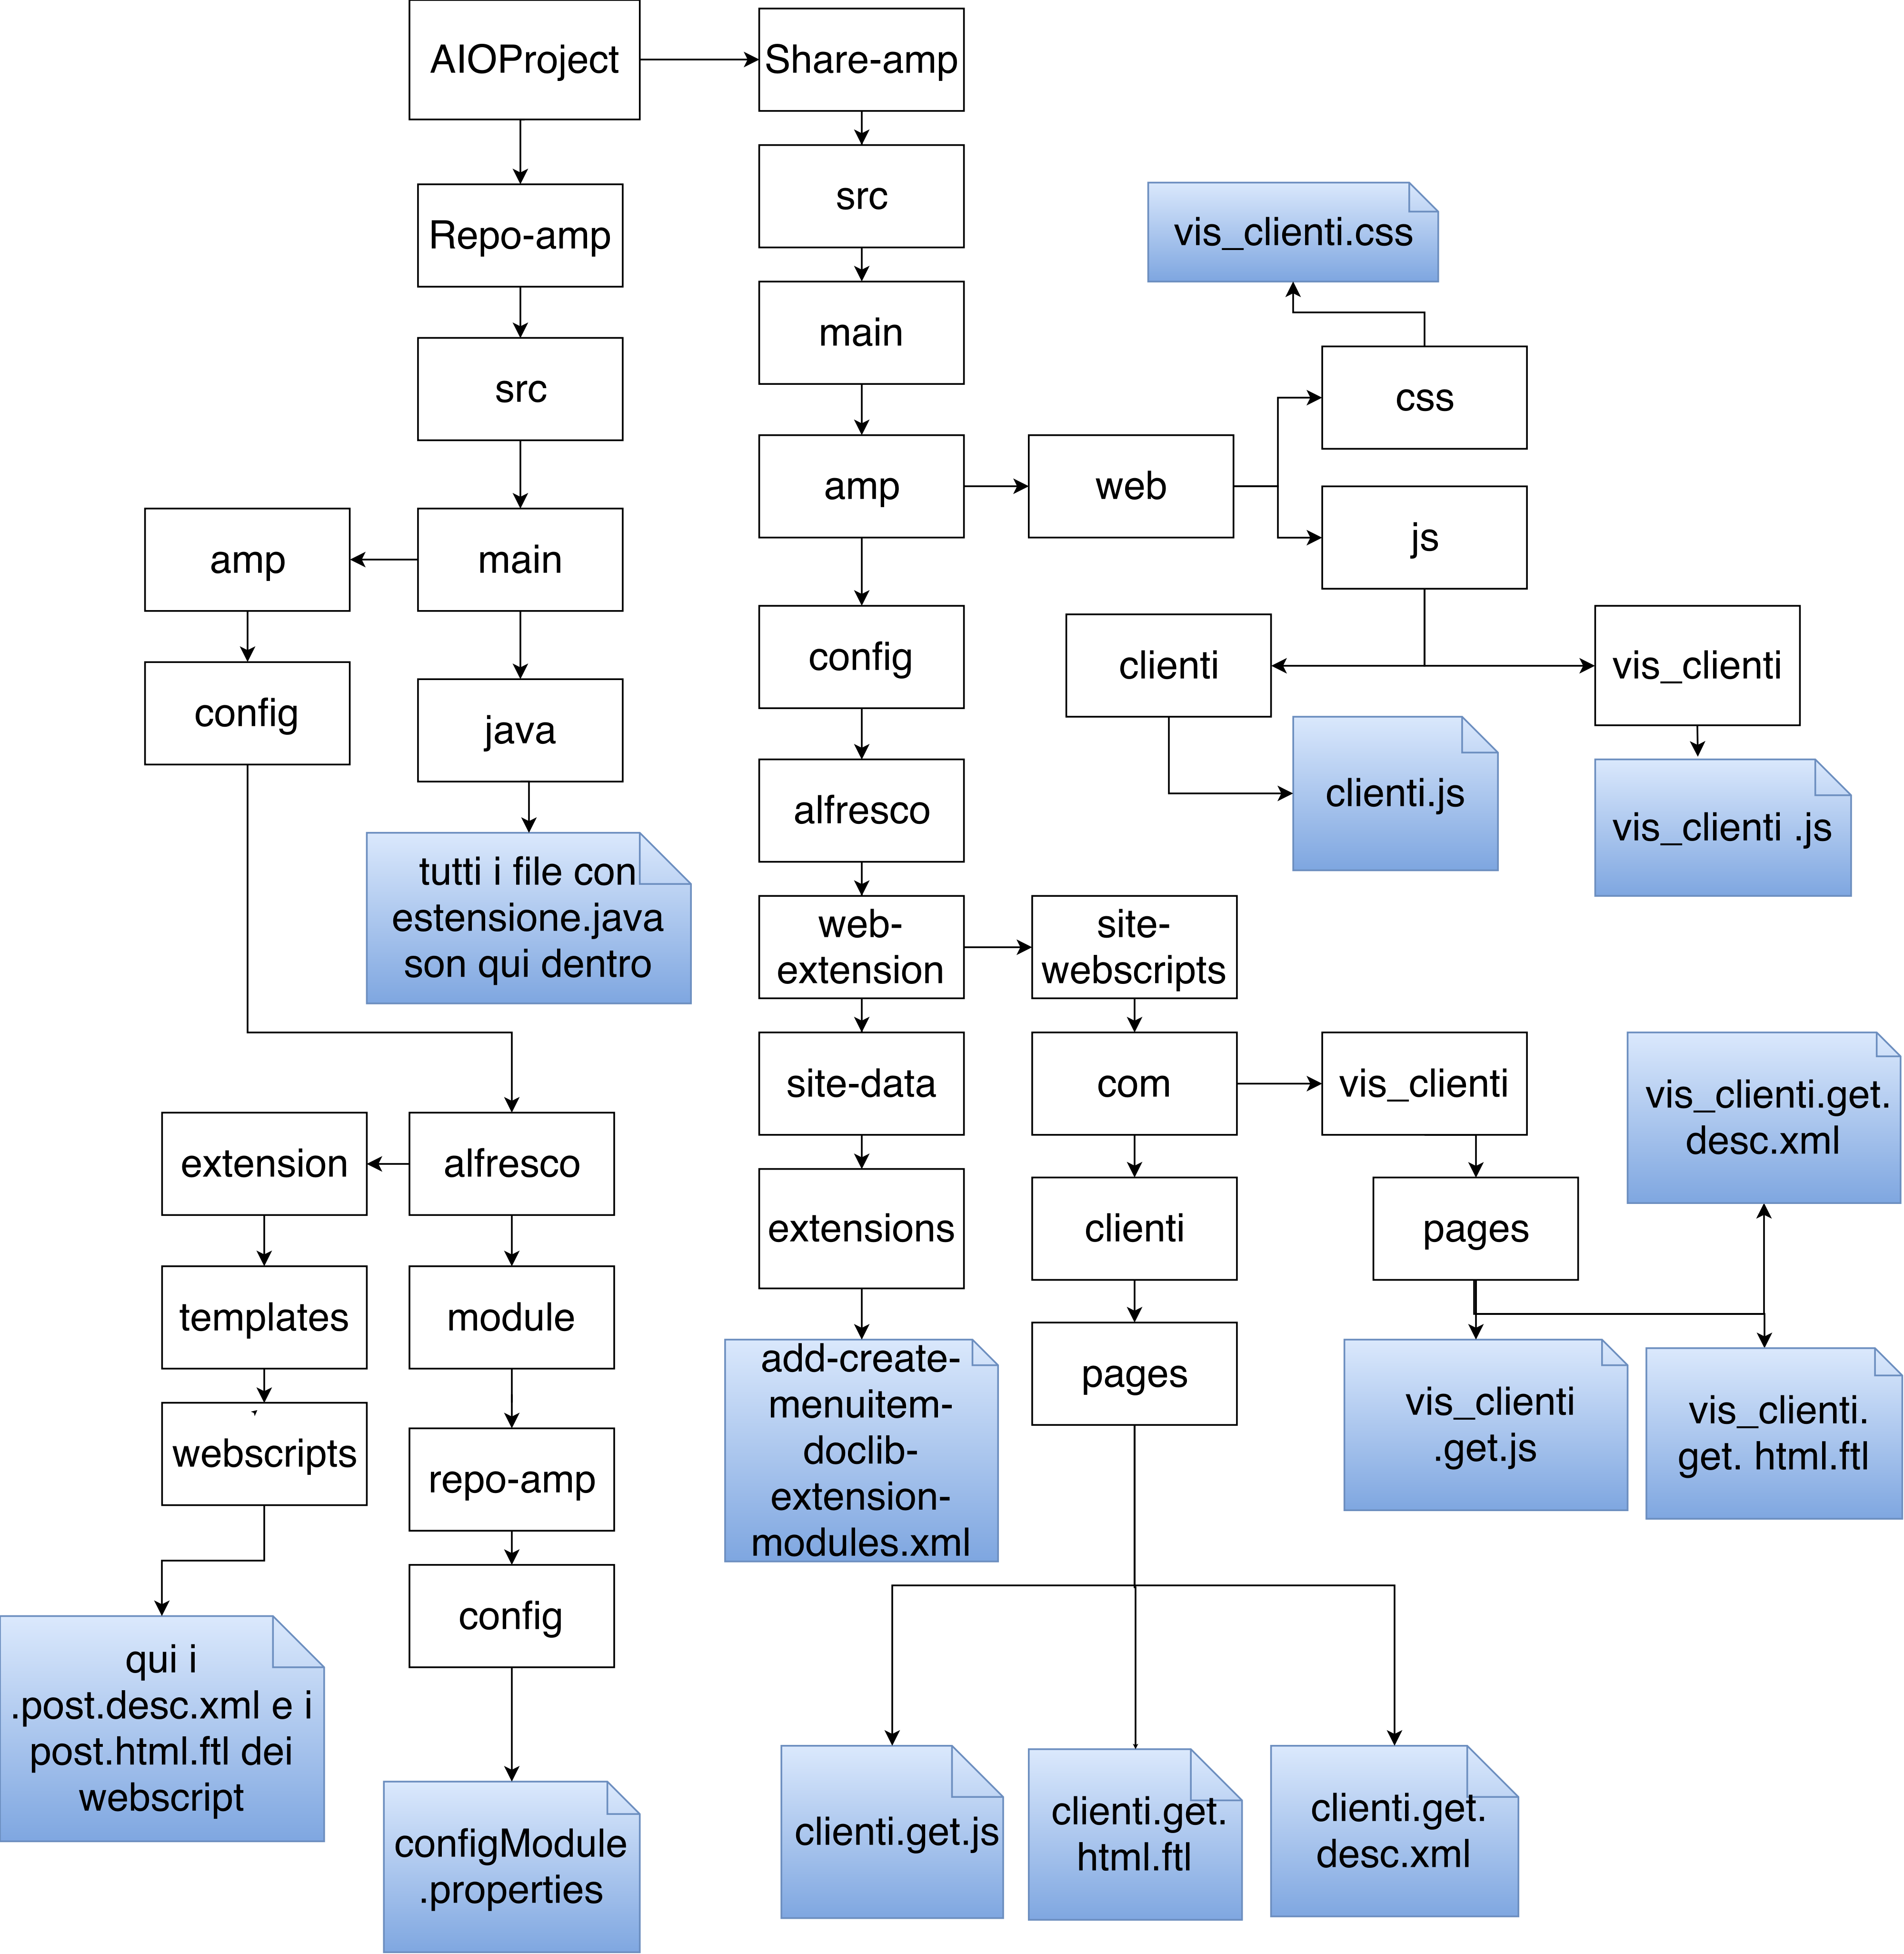
\includegraphics[width=\textwidth]{/diagrammi_cartelle/FolderClienti.png}
\caption{descrizione generale di quanto creato per il modulo relativo ai clienti\label{fig:cartelle-clienti}}
\end{figure}
\section{Implementazione delle funzionalità}
\subsection{Preparazione del DB}
Per preparare il DB bisogna innanzitutto creare un nuovo database.

Nel caso del progetto sviluppato in questo stage si è usato PostgreSQL, per i motivi già esposti.

È necessario quindi, per creare il database, spostarsi nella cartella di PostgreSQL tramite DOS e digitare il comando

\texttt{createdb -h localhost -p <porta> -U postgres <nome del db>}

Il passo successivo è quindi quello di crearvi una tabella, che verrà chiamata per comodità da adesso clienti.

La tabella ha la struttura che viene generata dal codice riportato nel listato \ref{lst:clienti-table}
\begin{lstlisting}[caption=codice per la creazione della cartella clienti, label=lst:clienti-table]
CREATE TABLE clienti
(
  identificativo text NOT NULL,
  name text NOT NULL,
  piva text NOT NULL,
  descr text,
  datainizio text NOT NULL,
  datafine text,
  id bigserial NOT NULL,
  CONSTRAINT clienti\_pkey PRIMARY KEY (id)
  CONSTRAINT clienti\_identificativo\_name\_piva\_descr\_datainizio\_datafine\_key UNIQUE (identificativo, name, piva, descr, datainizio, datafine)
)
\end{lstlisting}
Nel creare la tabella è importante prestare attenzione al fatto che l'owner della tabella debba essere il medesimo che è stato settato nelle properties.
L’ultimo vincolo è necessario per non avere record che differiscano solo per id.
In particolare si è scelto di tenere le date in formato testuale per rendere il db compatibile a diverse implementazioni sulla rappresentazione della data, e si è scelto di usare come chiave primaria un id chiamato bigserial, in quanto più resistente ad una eventuale estensione dei campi della tabella e più comodo da utilizzare, dal momento che, per le caratteristiche del bigserial, si è certi che l’ultima versione di un record è quella con l’id più alto, quindi per prendere l’ultima versione di un cliente di un determinato  identificativo basta eseguire la query \texttt{select * from clienti where id = (select max(id) from clienti where identificativo='param1')}. Si è cercato di non utilizzare viste o altri strumenti particolari per evitare di essere troppo dipendenti dalla piattaforma.



\subsection{Creazione della parte share}

È quindi stato necessario creare le pagine share e le pagine repo, oltre ai bean di collegamento per poter rendere accessibile il web script. Si è adottato il metodo POST in tutti quante le invocazioni, in quanto è più sicuro e permette lo scambio di una maggiore quantità di dati.

Si è aggiunta innanzitutto una nuova voce di menu aggiungendo il file \texttt{add-create-menuitem-doclib-extension-modules.xml}, il cui contenuto è riportato nel listato \ref{lst:doclib}
\begin{lstlisting}[language=XML,caption=add-create-menuitem-doclib-extension-modules.xml, label=lst:doclib]
<extension>
    <modules>
        <!-- This module is dependent on the custom content model setup in the repo-amp module -->
        <module>
            <id>Add a new menu item to Create... menu in DocLib</id>
            <version>1.0</version>
            <auto-deploy>true</auto-deploy>
            <configurations>
                <config evaluator="string-compare" condition="DocumentLibrary">
                    <create-content>
                        <content id="text-label-clienti" label="Crea nuovo cliente" icon="text" type="pagelink">
                            <param name="page">hdp/ws/clienti</param>
                        </content>
                    </create-content>
                </config>
                            </configurations>
        </module>
    </modules>
</extension>
\end{lstlisting}

Per ulteriore documentazione si faccia riferimento a al relativo capitolo nella documentazione di Alfresco \footcite{site:alfresco-doclib}

Le pagine includono inoltre nell’HTML la richiesta di JQuery, mediante le linee descritte nel listato \ref{JQuery}
\begin{lstlisting}[language=HTML, caption=inclusione JQuery, label=JQuery]
<script src="https://ajax.googleapis.com/ajax/libs/jquery/1.12.4/jquery.min.js"></script>
\end{lstlisting}

\subsubsection{Pagina clienti}

È la pagina di inserimento di un nuovo cliente ed è composta da un semplice form.
È composta dai seguenti file:
\begin{itemize}
\item \texttt{clienti.get.desc.xml}, implementato come descritto nel \hyperref[cap:architettura]{ quarto  capitolo}
\item\texttt{clienti.get.html.ftl }che contiene il codice html necessario a generare il form.
\item\texttt{clienti.get.js} che contiene le istruzioni necessarie a generare l’header. È necessario includere nell’html la linea \texttt{<@processJsonModel group="share"/>}.
\item \texttt{clienti.js,} incluso con la linea \texttt{<script src="\${url.context} / js / clienti / clienti.js"></script>}, che effettua i controlli javascript della pagina. In particolare alla pressione del pulsante di conferma viene fatto il controllo sui dati inseriti, cioè sulla correttezza della partita IVA, sul fatto che i campi obbligatori siano definiti, sul fatto che la data di fine sia successiva alla data di inizio. Inoltre si occupa di inoltrare la richiesta AJAX al web script \texttt{query\_processor.java} che sarà trattato successivamente. Se il web script riporta uno stato anomalo viene segnalato e così viene anche gestito il caso di inserimento di un identificativo già esistente.
\end{itemize}

\subsubsection{Pagina vis\_clienti}

La pagina vis\_clienti è la pagina di gestione dei clienti, ed è suddivisa nei file:
\begin{itemize}
\item \texttt{vis\_clienti.get.desc.xml} che funziona come descritto nel \hyperref[cap:architettura]{ quarto  capitolo}.
\item \texttt{vis\_clienti.get.html.ftl} che fornisce lo scheletro della pagina, che verrà poi popolata tramite richieste AJAX delle parti dinamiche.
\item \texttt{vis\_clienti.get.js}, che funziona come descritto prima.
\item \texttt{vis\_clienti.css}, incluso in maniera analoga al javascript come descritto prima e che definisce il CSS della pagina.
\item \texttt{vis\_clienti.js}, incluso come descritto prima
\end{itemize}
In particolare la pagina nella sua parte principale offre la lista degli identificativi dei clienti attivi e non, che è anche il nome con cui sono stati salvati nelle cartelle di Alfresco. Si è scelto questa rappresentazione in quanto è logicamente vicina alla struttura di Alfresco e sarà più facile in futuro implementare funzionalità quali la visualizzazione dei progetti del cliente.  I pulsanti dei clienti attivi e inattivi sono generati rispettivamente da \texttt{clients.java}  e  \texttt{inactive.java}  chiamati all’avvio della pagina tramite \texttt{window.onload} che si occupano di definire anche i giusti parametri che verranno poi utilizzati per popolare il form che consente l’aggiornamento dei dati di un particolare cliente. Il form è già presente nella pagina ma viene reso visibile da una opportuna funzione javascript che si occupa anche di popolare la tabella sottostante tramite una chiamata AJAX al web script \texttt{TablePageGenerator.java}, che si occupa di fornire la tabella e di iniettare il pulsante cancella e il pulsante  per definire  la data di fine del rapporto  con il corretto id. I pulsanti sono collegati a loro volta a \texttt{delete.java} e \texttt{update.java}, chiamati tramite opportune chiamate AJAX.

I messaggi di errore e di conferma sono gestiti dove possibile in JavaScript e dove non possibile, poiché la risposta dipende dal database o dal repository, tramite la risposta della chiamata AJAX

Per riassumere la pagina fa uso delle seguenti funzioni JavaScript:
\begin{itemize}
\item \texttt{set\_table(identificativo)} che si occupa di generare la tabella di un determinato cliente tramite richiesta AJAX
\item \texttt{detail(id,nome,pi,descr,datainizio,datafine)}che si occupa di settare 
E mostrare il dettaglio di un cliente
\item \texttt{controllaPIVA(pi)} che esegue semplicemente  il controllo della partita IVA
\item \texttt{sendRequest()} Che invia la richiesta AJAX di aggiornamento di un determinato cliente
\item \texttt{set\_data\_fine(ID)} che setta la data di fine di un determinato record di un cliente tramite richiesta AJAX
\item \texttt{cancella(key)} che fa la richiesta tramite AJAX di cancellazione di un record con un determinato ID
\item \texttt{up()} che popola la pagina con i pulsanti dei clienti, tramite richiesta AJAX.
\item \texttt{vai(name)} che reindirizza alla cartella con dato nome.
\end{itemize}
Sono presenti altre funzioni che svolgono compiti banali quale la codifica e decodifica di entità, per garantire il funzionamento della pagina nel caso i record contengano caratteri speciali



\subsection{Creazione della parte repo}
\subsubsection{Creazione delle variabili del modulo}
Per rendere possibile la modifica di alcune configurazioni anche dopo che il modulo è stato installato in alfresco, si è provveduto a creare un file in \texttt{configModule.properties}, Accessibile da Java aggiungendo al codice le linee mostrate nel listato \ref{lst:properties}
\begin{lstlisting}[language=Java, caption= inclusione delle properties, label=lst:properties]
private static Properties properties=new Properties();

public static final String getValue(String value) {
		return properties.getProperty(value);
	}
	
properties.load(getClass().getResourceAsStream("/alfresco/module/AIOProject-repo-amp/config/configModule.properties"));
\end{lstlisting}
Questo permette quindi di recuperare le variabili, che si è cercato di documentare direttamente sul codice tramite nomi significativi e una breve descrizione. Il codice è riportato nel listato \ref{lst:clienti-properties}
\begin{lstlisting}[caption=contenuto di configModule.properties,label=lst:clienti-properties]
#query configuration
queryselection=select id,name, piva, datainizio, datafine, descr from clienti where identificativo='param1' order by id
querylastversion=select * from clienti where id = (select max(id) from clienti where identificativo='param1')
queryselectactive=select distinct identificativo from clienti where NOT (datafine IS NOT NULL)
queryselectnotactive=select distinct identificativo from clienti where datafine IS NOT NULL and identificativo not in (select distinct identificativo from clienti where NOT (datafine IS NOT NULL))
#do not use values in the form paramX! They may be sobstituted!
queryselectionwithclause=select param1 from param2 where param3
queryinsertion=insert into param1 values ('param2','param3','param4', 'param5', 'param6', 'param7')
queryupdate=UPDATE param1 SET param2 = 'param3' WHERE id = 'param4';
querydelete=DELETE FROM param1 WHERE id = 'param2';
#set param1 in the previous query
querytable=Clienti
#server configuration
serverip=127.0.0.1
serverid=alfresco
serverpassword=admin
serverport=5432
servername=<nome del database creato>
servertype=postgresql
serverconnector=jdbc
#path in lucene, in the form of PATH:/"/{directory}, the "/"" character is needed 
#because without it it will be escaped by java, java alone puts the final " so 
#you must not put it when you write the query
installationpath=PATH:/"/app:company_home/st:sites/cm:er/cm:documentLibrary/cm:_x0030_2_x0020_-_x0020_Clients
#down here you can put the names for the folder that are in the client subdirectory
folder.one=01 - Projects
folder.two=02 - General Contracts
folder.three=tre
folder.four=quattro
folder.five=cinque
\end{lstlisting}
Come si vede dove necessario si è cercato di parametrizzare le funzioni.


\subsubsection{Creazione dei web script}
Come già accennato, le pagine in share per il loro completo funzionamento necessitano di web script di supporto, per interrogare il database e generare le tabelle contenenti i dati.  Tutti quanti estendono la classe AbstractWebScript, sono contattabili tramite POST e fanno uso del JDBC per contattare il server remoto dove è presente la tabella. Il file .properties descritto prima permette di cambiare secondo le necessità la configurazione della connessione, definita nella riga riportata nel listato \ref{lst:java-jdbc}
\begin{lstlisting}[language=Java, caption=connesione tramite JDBC, label=lst:java-jdbc]
connection=DriverManager.getConnection((connector+":"+type+"://"+ip+":"+port+"/"+server),id,password);
\end{lstlisting}
Che sono i parametri definiti nel paragrafo query configuration del .properties

I Web Script sono poi registrati nel file \texttt{webscript-context.xml} secondo le modalità già descritte.

Per comodità nella chiamata l’indirizzo è stato settato con lo stesso nome della funzione java ad esso corrispondente. Inoltre alcuni  accettano parametri in JSON definiti in coppie \texttt{{key:value}} in un JSonObject

Passiamo ora in rassegna i vari web script implementati, in ordine alfabetico.
\paragraph{clients.java}
Questo web script, situato in \texttt{clients.java} e dalla pagina definita in \texttt{clients.post.desc.xml} e in \texttt{clients.post.html.ftl}, si occupa di generare i pulsanti necessari a visualizzare poi la pagina di dettaglio per un utente attivo. Si occupa quindi di interrogare il database e di definire di conseguenza i parametri dei pulsanti e il loro nome, che chiamano uno la funzione \texttt{detail(id,nome,pi,descr,datainizio,datafine)},e l’altro la funzione \texttt{vai(name)}. Si appoggia sulla query definita in queryselectactive per selezionare gli utenti attivi, percorrendo poi il result set per di volta in volta assegnare i parametri.
Viene chiamato senza parametri.
La classe si compone delle seguenti funzioni:
\begin{itemize}
\item \texttt{getValue(String value)}, che recupera una property con una data value.
\item \texttt{inizialize\_values ()}, che inizializza le variabili utilizzate, recuperandole dalle properties.
\item \texttt{public void execute(WebScriptRequest req, WebScriptResponse res)} metodo obbligatorio che si può intendere come il metodo che viene invocato alla chiamata Ajax del web script e che contiene le istruzioni per gestirla.
\item \texttt{execute(Connection con, String query, WebScriptResponse res)}, metodo che esegue la query.
\item \texttt{writedata(ResultSet rs, String result, Connection con)}, metodo che si occupa di ritornare il codice html necessario a generare i pulsanti dei clienti attivi
\end{itemize}
\paragraph{delete.java}
Questo web script, situato in \texttt{delete.java} e dalla pagina definita in \texttt{delete.post.desc.xml} e in \texttt{delete.post.html.ftl}  si occupa semplicemente di cancellare un elemento che abbia un determinato id, fornito come parametro della chiamata. Si appoggia sulla query definita alla voce querydelete.
La classe si compone delle seguenti funzioni:
\begin{itemize}
\item \texttt{getValue(String value)}, che recupera una property con una data value
\item \texttt{inizialize\_values ()}, che inizializza le variabili utilizzate, recuperandole dalle properties.
\item \texttt{public void execute(WebScriptRequest req, WebScriptResponse res)} metodo obbligatorio che si può intendere come il metodo che viene invocato alla chiamata Ajax del web script e che contiene le istruzioni per gestirla.
\item \texttt{execute(Connection con, String query)}, metodo che esegue la query di delete di un dato record del database.
\end{itemize}
\paragraph{inactive.java}
Questo web script, situato in \texttt{inactive.java} e dalla pagina definita in \texttt{inactive.post.desc.xml} e in \texttt{inactive.post.html.ftl} si occupa di generare i pulsanti necessari a visualizzare poi la pagina di dettaglio per un utente non più attivo. Si occupa quindi di interrogare il database e di definire di conseguenza i parametri del pulsante e il suo nome, che chiama la funzione \texttt{detail(id,nome,pi,descr,datainizio,datafine)}. Si appoggia sulla query definita in queryselectnotactive per selezionare gli utenti non attivi. Percorrendo poi il result set per di volta in volta assegnare i parametri.
Viene chiamato senza parametri.
La classe si compone delle seguenti funzioni:
\begin{itemize}
\item \texttt{getValue(String value)}, che recupera una property con una data value
\item \texttt{inizialize\_values ()}, che inizializza le variabili utilizzate, recuperandole dalle properties.
\item \texttt{public void execute(WebScriptRequest req, WebScriptResponse res)} metodo obbligatorio che si può intendere come il metodo che viene invocato alla chiamata Ajax del web script e che contiene le istruzioni per gestirla.
\item \texttt{execute(Connection con, String query, WebScriptResponse res)}, metodo che esegue la query.
\item \texttt{writedata(ResultSet rs, String result, Connection con)}, metodo che si occupa di ritornare il codice html necessario a generare i pulsanti dei clienti non attivi.
\end{itemize}
Si è deciso di renderla autonoma rispetto a clients per consentire una migliore estensione ad ulteriori eventuali funzionalità.
\paragraph{query\_processor.java}
Questo web script, situato in \texttt{query\_processor.java} e dalla pagina definita in \texttt{query\_processor.post.desc.xml} e in \texttt{query\_processor.post.html.ftl} . Si occupa di inserire un oggetto nel database, utilizzando la query definita in  queryinsertion e deve essere chiamato con i seguenti parametri:
\begin{itemize}
\item ID:l’identificativo del cliente,
\item Nome:il nome esteso del cliente,
\item Piva:la partita iva del cliente,
\item Descr:una descrizione generica,
\item Datainizio:la data di inizio del rapporto,
\item Datafine:la data di fine del rapporto(se non presente, verrà settata a null),
\item Mode:1=inserimento con la creazione delle cartelle, 2=inserimento senza creazione di cartelle ,
\item Box1:flag per la creazione della cartella di nome definito in folder.one,
\item box2:flag per la creazione della cartella di nome definito in folder.two,
\item box3:flag per la creazione della cartella di nome definito in folder.three,
\item box4:flag per la creazione della cartella di nome definito in folder.four,
\item box5:flag per la creazione della cartella di nome definito in folder.five,
\end{itemize}
Lo script si appoggia, oltre al JDBC per l’inserimento nel database, sulla \gls{API} di Alfresco 
FileFolderService per creare la gerarchia di cartelle corrispondente, di permissionservice per settare i permessi di accesso alle cartelle (per il momento codificati nel Java e non configurabili dopo l’installazione se non mediante l’editor dei permessi di Alfresco)
E fa utilizzo anche nodeservice, un altro elemento dell'\gls{API}, per settare la descrizione della cartella principale.
Per includere il serviceregisty, necessario per accedere alla \gls{API} di Alfresco, è necessario, oltre a specificare  nel bean, il cui funzionamento è stato già descritto, tramite le righe mostrate nel listato \ref{lst:service-registry}
\begin{lstlisting}[language=XML,label=lst:service-registry,caption=inclusione del service registry nel bean]
        <property name="serviceRegistry">
          <ref bean="ServiceRegistry" />
      </property>
\end{lstlisting}
E poi nel codice java con l’aggiunta di quanto mostrato alla figura \ref{lst:service-registry-java}
\begin{lstlisting}[language=Java,label=lst:service-registry-java,caption=inclusione del service registry nel bean]
import org.alfresco.service.ServiceRegistry;

private ServiceRegistry serviceRegistry;

public void setServiceRegistry(ServiceRegistry serviceRegistry) {
		this.serviceRegistry = serviceRegistry;
	}
\end{lstlisting}
Ritorna una stringa di risultato dove è specificato l’esito dell’operazione.
La classe si compone delle seguenti funzioni:
\begin{itemize}
\item \texttt{setServiceRegistry(ServiceRegistry serviceRegistry)}, che inizializza il parametro per il service registry di Alfresco. È richiesto obbligatoriamente da Alfresco se si vogliono utilizzare le sue funzionalità
\item \texttt{getValue(String value)}, che recupera una property con una data value
\item \texttt{inizialize\_values ()}, che inizializza le variabili utilizzate, recuperandole dalle properties.
\item \texttt{public void execute(WebScriptRequest req, WebScriptResponse res)} metodo obbligatorio che si può intendere come il metodo che viene invocato alla chiamata Ajax del web script e che contiene le istruzioni per gestirla.
\item \texttt{execute(Connection con, String query)}, metodo che esegue la query.
\item \texttt{create\_folder\_tree(String ID, String descr,Boolean box1, Boolean box2, Boolean box3, Boolean box4, Boolean box5)}, metodo che si occupa di creare le cartelle relative ad un nuovo cliente, di settarne i permessi e di settare la descrizione della cartella padre.
\end{itemize}
\paragraph{TablePageGenerator.java}
Questo web script, situato in \texttt{TablePageGenerator.java} e dalla pagina definita in \texttt{TablePageGenerator.post.desc.xml} e in \texttt{TablePageGenerator.post.html.ftl}  si occupa di generare la tabella dello storico di un determinato codice cliente, fornito come parametro della chiamata AJAX. Si appoggia sulla query definita alla voce queryselection.
Il web script si occupa di generare il codice della tabella e di iniettare i giusti parametri nel pulsante per cancellare, e, nel caso la data di fine non sia stata settata, anche di generare il pulsante per la modifica della data di fine rapporto.
La classe si compone delle seguenti funzioni:
\begin{itemize}
\item \texttt{getValue(String value)}, che recupera una property con una data value
\item \texttt{inizialize\_values ()}, che inizializza le variabili utilizzate, recuperandole dalle properties.
\item \texttt{public void execute(WebScriptRequest req, WebScriptResponse res)} metodo obbligatorio che si può intendere come il metodo che viene invocato alla chiamata Ajax del web script e che contiene le istruzioni per gestirla.
\item \texttt{execute(Connection con, String query, WebScriptResponse res)}, metodo che esegue la query.
\item \texttt{dumpData(ResultSet rs, String result)}, metodo che si occupa di ritornare il codice html necessario a generare la tabella dello storico di un cliente.
\end{itemize}
\paragraph{update.java}
Questo web script, situato in \texttt{update.java} e dalla pagina definita in \texttt{update.post.desc.xml} e in \texttt{update.post.html.ftl}  si occupa semplicemente di cancellare un elemento che abbia un determinato id, un campo da aggiornare e un valore con cui aggiornarlo,  forniti come parametro della chiamata. Si appoggia sulla query definita alla voce queryupdate.
La classe si compone delle seguenti funzioni:
\begin{itemize}
\item \texttt{getValue(String value)}, che recupera una property con una data value
\item \texttt{inizialize\_values ()}, che inizializza le variabili utilizzate, recuperandole dalle properties.
\item \texttt{public void execute(WebScriptRequest req, WebScriptResponse res)} metodo obbligatorio che si può intendere come il metodo che viene invocato alla chiamata Ajax del web script e che contiene le istruzioni per gestirla.
\item \texttt{executeupdate(Connection con, String query)}, metodo che esegue la query di update della data di fine di un dato record del database.
\end{itemize}

\section{Aspetto estetico}
Per il lato estetico si è reso necessario contattare il team di grafici che lavora presso l'azienda per ottenere un aspetto gradevole e che si allineasse con quanto già presente in Alfresco. Sono stati quindi forniti dei mockup delle varie componenti ed è stato chiesto allo stagista di riprodurre tale aspetto in Alfresco.
\subsection{Risultati raggiunti}
Nella figura \ref{fig:cliente-insert} si può vedere l'aspetto della pagina di inserimento di un nuovo cliente, mentre nelle figure \ref{fig:clienti-lista} e \ref{fig:cliente-detail} vi è la pagina dedicata alla visualizzazione e modifica dei clienti inseriti. la modifica della data di fine rapporto e la conferma per la cancellazione sono state implementate tramite un pop-up JQuery.
\begin{figure}[!ht]
\centering
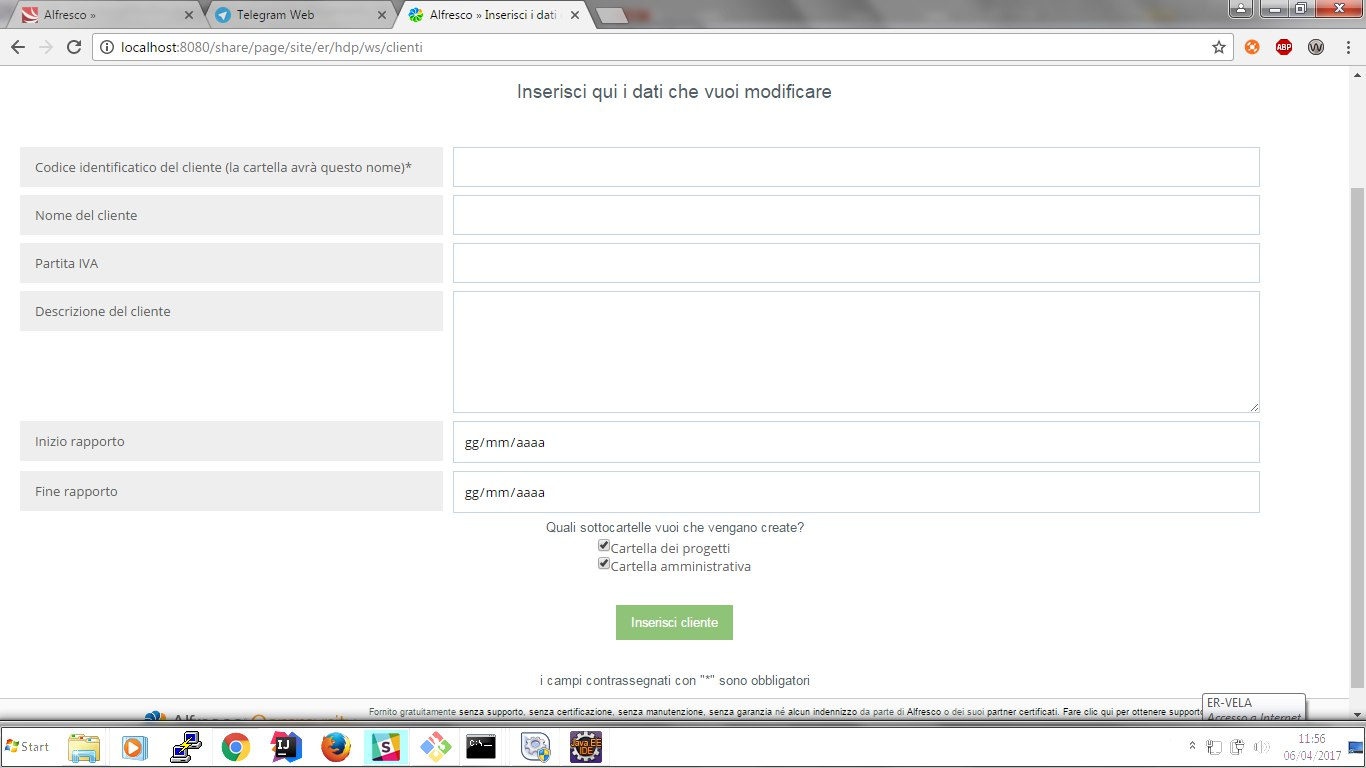
\includegraphics[width=\textwidth]{nuove_immagini/cliente-insert}
\caption{pagina di inserimento di un nuovo cliente\label{fig:cliente-insert}}
\end{figure}
\begin{figure}[!ht]
\centering
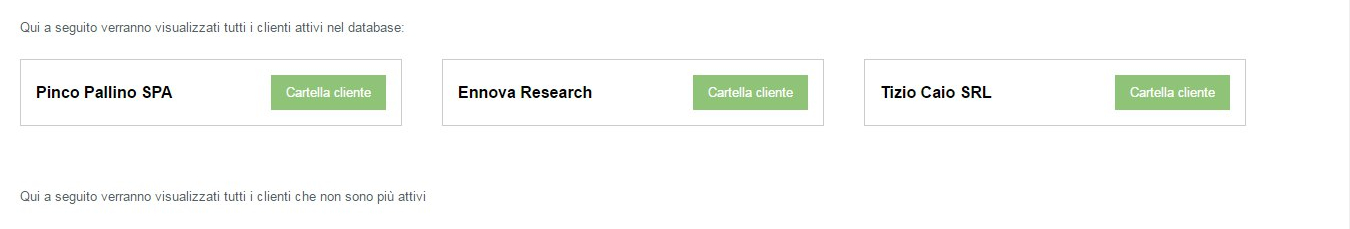
\includegraphics[width=\textwidth]{nuove_immagini/clienti-lista}
\caption{pagina di visualizzazione dei clienti nel database\label{fig:clienti-lista}}
\end{figure}
\begin{figure}[!ht]
\centering
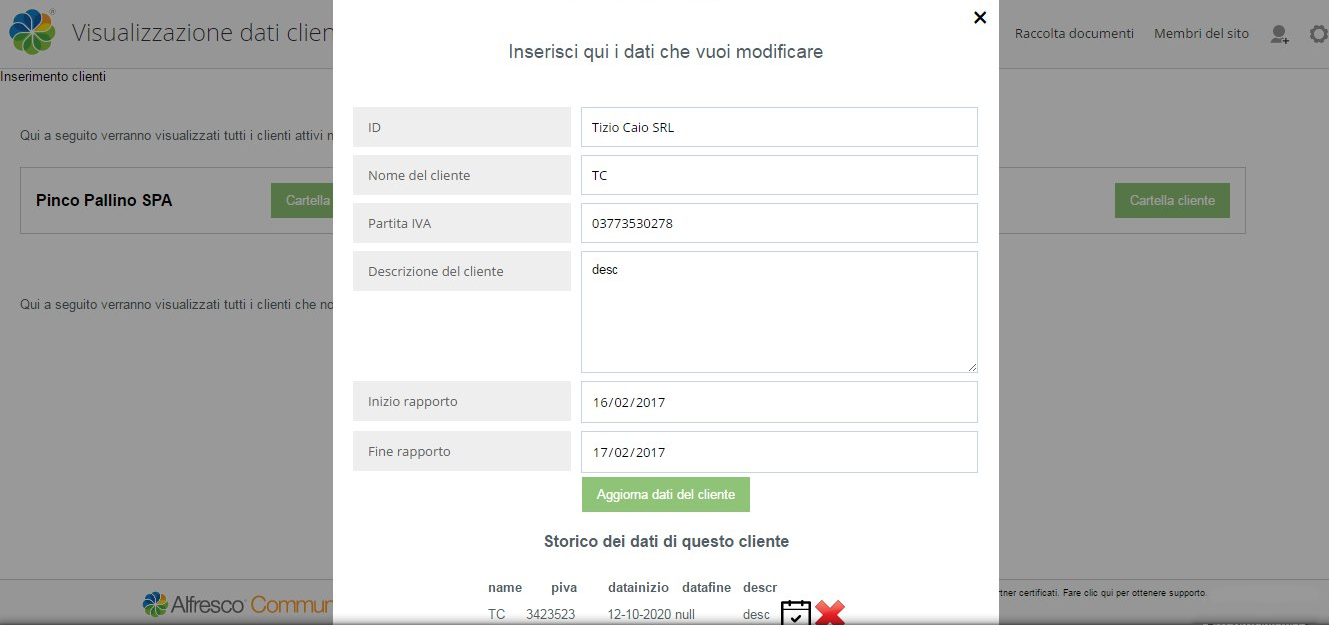
\includegraphics[width=\textwidth]{nuove_immagini/cliente-detail}
\caption{pagina di dettaglio di un cliente \label{fig:cliente-detail}}
\end{figure}